
\subsection{General Equation of Motion}
The state of the electron hydrogen
system at a given time can be completely
characterised by its density
matrix.
Working in the interaction
picture, a general density matrix
\(\hat{\rho}(t)\) time evolves according
to the von Neumann equation~\cite{TP2_Notes}.
\begin{equation}
    \frac{d\hat{\rho}_t(t)}{dt} =
    -i [\hat{H}_{int}(t), \hat{\rho}_t(t)]
    \label{eqn:density equation of motion}
\end{equation}
which can be integrated to give
\begin{equation}
    \hat{\rho}_t(t) =
    \hat{\rho}_t(0)
    - i \int_0^t ds
        [\hat{H}_{int}(s), \hat{\rho}_t(s)]
    \label{eqn:integrated density equation of motion}
\end{equation}
We can expand this equation of motion
to second order in the interaction
by substituting \cref{eqn:integrated density equation of motion}
into \cref{eqn:density equation of motion}
twice to give
\begin{equation}
    \frac{d\hat{\rho}_t(t)}{dt} =
    -i [\hat{H}_{int}(t), \hat{\rho}_t(0)]
    - \int_0^t ds
        [\hat{H}_{int}(s),
            [\hat{H}_{int}(s), \hat{\rho}_t(t)]]
    +\mathcal{O}({\hat{H}_{int}}^3)
    \label{eqn:second order eqn of motion}
\end{equation}
It is possible to reduce this to
an equation of motion
describing just the system by taking
a trace over the environment~\cite{Manzano_2020}
\begin{equation}
    \hat{\rho}(t) =
    -i Tr_e[\hat{H}_{int}(t), \hat{\rho}_t(0)]
    - \int_0^t ds
    Tr_e[\hat{H}_{int}(s),
    [\hat{H}_{int}(s), \hat{\rho}_t(t)]]
    \label{eqn:density motion before redfield approximation}
\end{equation}
where \(\hat{\rho}(t) = Tr_e[\hat{\rho}_t(t)]\)
is the density operator of the system.
Using a clever re-definition of the interaction
Hamiltonian~\cite{Manzano_2020} it
is possible to show that the first
term gives no contribution to the
overall dynamics of the system.

\subsection{The Redfield Assumption}\label{sec:the redfield assumption}
To arrive at the Redfield equation
we first make the assumption that the
system and surrounding density
matrix is completely
decoupled~\cite{theory_open_quantum_systems},
allowing us to write
\begin{equation}
    \hat{\rho}_t(t) = \hat{\rho}(t) \otimes \hat{\rho}_E(t)
\end{equation}
where \(\hat{\rho}_E(t)\), the
density matrix of the environment,
is taken as a purely statistical ensemble.
Under the Markov approximation
we can extend the upper limit
of \cref{eqn:density motion before redfield approximation}
to \(\infty \), arriving at the Redfield
equation
\begin{equation}
    \dot{\hat{\rho}}(t) =
    - \int_0^{\infty} ds
    Tr_{E}[\hat{H}_{int}(t),
            [\hat{H}_{int}(s-t),
                    \hat{\rho}(t) \otimes \hat{\rho}_E(t)]]
\end{equation}
Separating out the interaction hamiltonian
into system and surroundings according
to~\cref{eqn:split interaction hamiltonian}
\begin{align}
    \hat{H}_{int} & = \sum_{i,j} \hat{S}_{i,j} \hat{E}_{i,j}
\end{align}
we can simplify the form of this equation\cite{Manzano_2020} to give
\begin{equation}
    \dot{\hat{\rho{}}}(t) = \begin{aligned}[t]
        \sum_{i,j,k, l} &
        \exp{(-i(\omega_{i,j}-\omega_{k,l})t)}
        \Gamma_{i,j;k, l}(\omega_{k,l})
        [S_{k, l}\hat{\rho}(t),
        S^\dagger_{i,j}]  \\
        +               &
        \exp{(i(\omega_{i,j}-\omega_{k,l}))}
        \Gamma^*_{k, l; i,j}(\omega_{i,j})
        [S_{k, l},
            \hat{\rho}(t) S^\dagger_{i,j}]
    \end{aligned} \label{eqn:redfield equation gamma form}
\end{equation}
where \(\Gamma \) is the
Lindblad rate constant given by
\begin{equation}
    \Gamma_{i,j, k,l}(\omega) =
    \int_0^\infty{}{
    ds \exp{(i\omega{}s)}
    Tr_{E}[E^\dagger_{i,j}(t)E_{k,l}(t-s)\rho_E(0)]
    }\label{eqn:gamma definition}
\end{equation}

\subsection{The Lindblad Equation}\label{sec:lindblad equation}
To obtain the Lindblad equation
we need to apply the rotating
wave approximation to
\cref{eqn:redfield equation gamma form}.
We first expand out the commutators
in \cref{eqn:redfield equation gamma form}
\begin{align}
    \bra{m}[S_{k, l}\hat{\rho}(t),
    S^\dagger_{i, j}] \ket{n}              & =
    \sum_{\alpha, \beta} \rho_{\alpha, \beta} [
        \delta_{m, k}\delta_{l, \alpha}
        \delta_{\beta, j}\delta_{i, n}
        -\delta_{m, j}\delta_{i, k}
    \delta_{l, \alpha}\delta_{\beta, n}]       \\
    \bra{m}[S_{k, l},
    \hat{\rho}(t)S^\dagger_{i, j}] \ket{n} & =
    \sum_{\alpha, \beta} \rho_{\alpha, \beta} [
        \delta_{m, k}\delta_{l, \alpha}
        \delta_{\beta, j}\delta_{i, n}
        -\delta_{m, \alpha}\delta_{\beta, j}
        \delta_{i, k}\delta_{l, n}]
\end{align}
which we use to obtain an expanded
form
\begin{equation}
    \bra{m}\dot{\hat{\rho}}(t) \ket{n} = \begin{aligned}[t]
        \sum_{i,j,k, l, \alpha, \beta} &
        \exp{(-i\Delta{}Et)}
        \Gamma_{i,j;k, l}(\omega_{k,l})
        \rho_{\alpha, \beta} [\dots]                          \\
        +                              & \exp{(i\Delta{}E t)}
        \Gamma^*_{k, l; i,j}(\omega_{i,j})
        \rho_{\alpha, \beta} [\dots]
    \end{aligned}
\end{equation}
where \(\Delta{}E = \omega_{i,j}-\omega_{k,l}\).
The rotating wave approximation
limits us to two cases
\begin{itemize}
    \item \(i=j\), \(k=l\)
    \item \(i=k\), \(j=l\)
\end{itemize}
which is imposed using the expression
\(\delta_{i,j}\delta_{k,l}
+ \delta_{i,k}\delta_{j,l}
- \delta_{i,j}\delta_{k,l}
\delta_{i,k}\). This
leads us to the
general expression (\cref{eqn:cross terms density matrix evolution})
\begin{equation}
    \bra{m}\dot{\hat{\rho}}(t) \ket{m}  =
    2 \sum_{n\neq m}
    [  \Gamma_{m,n;m, n}(\omega_{m,n})\rho_{n, n}
        - \Gamma_{n,m;n, m}(\omega_{n,m})\rho_{m, m}]
\end{equation}
where we sum over all neighbouring
sites \(n \neq m\). Note that
the off diagonal
terms vanish assuming the
density matrix is initially
purely diagonal. A full derivation
can be found in
\cref{app:redfield to lindblad}.



\subsection{Lindblad Rate Constant}
Using \cref{eqn:gamma definition}
we can calculate the value of
the Lindblad rate constant \(\Gamma \).
If we assume the electrons
are initially in a purely
statistical ensemble the
density matrix is given
by\cite{sakurai_napolitano_2020}
\begin{equation}
    \rho_E(0) = \sum_{\{N(k)\}}
    P(\{N(k)\})
    \ket{N(k)} \bra{N(k)}
\end{equation}
using the definition
of \(\hat{E}_{i,j}\) given
in \cref{sec:simplified interaction}
we can
take the trace over the
environment (see \cref{app:calculating gamma})
\begin{equation}
    Tr_E[\dots]  = \begin{aligned}[t]
        \sum_{\substack{\{N(k)\}                             \\
        k_1,s^1,k_2,s^2                                      \\
                k_3,s^3,k_4,s^4 }}
         & P(\{N(k)\}) V_{i,j} V_{k,l}                       \\
         & \exp{(i(E_1 - E_2) t)} \exp{(i(E_3 - E_4) (t-s))} \\
         & \bra{N(k)}
        \hat{b}_{k_1,s^1}^\dagger{} \hat{b}_{k_2,s^2}
        \hat{b}_{k_3,s^3}^\dagger{} \hat{b}_{k_4,s^4}
        \ket{N(k)}
    \end{aligned}
\end{equation}
where \( \{N(k)\} \) is the set of
all possible occupations, and
the boltzmann
probability associated with a
given state is
\(P(\{N(k)\}) = \exp{(-\beta{}(E-\mu N))}\).
The trace is only non zero in two
cases
\begin{itemize}
    \item \(k_1=k_2, s^1=s^2\),
          \(k_3=k_4, s^3=s^4\)
    \item \(k_1=k_4, s^1=s^4\),
          \(k_3=k_2, s^3=s^2\) but
          \(k_1\neq{}k_2, s^1\neq{}s^2\)
\end{itemize}
and we can therefore obtain the
simplified form of the trace
\begin{equation}
    Tr_E[\dots] = \begin{aligned}[t]
        \sum_{k_1,s^1,k_3,s^3 }
         & V_{i,j} V_{k,l} [
                N_1 N_3
                + N_1 (1 - N_3) \exp{(-i(E_3 - E_1)s)}]
    \end{aligned}
\end{equation}
Integrating over \(s\) we obtain
an additional constant on the
wavevectors, and after
converting the sum into
an integral and re-adsorbing
the power of \(L^3\) into the
definition of \(V_{i,j}\)
(see \cref{sec:simplified interaction})
we find
\begin{align}
    \Gamma_{i,j, k,l}(\omega) & =\begin{aligned}[t]
        \sum_{s^1,s^3} \int &
        \frac{d^3\vec{k}_1}{{(2\pi)}^3}
        \frac{d^3\vec{k}_3}{{(2\pi)}^3}
        V_{i,j} V_{k,l} [
        N_1 N_3 \delta_{w, 0} \frac{m_e}{\sqrt{k_3^2}} \\
                            & + N_1 (1 - N_3)
                \frac{m_e}{\sqrt{k_1^2 - 2m_e\omega}}
                \delta({k_3 \pm \sqrt{k_1^2 + 2m_e\omega}}) ]
    \end{aligned}\label{eqn:gamma integral form}
\end{align}
The first term is divergent, however
since we find no terms in the Redfield
equation with \(\omega = 0\)
it does not contribute to tunneling.
We evaluate the second term
by expanding the integrand about the fermi
wavevector
\begin{equation}
    \frac{k_1 ^ 2 k_3 ^ 2 N_1 (1 - N_3)}
    {\sqrt{k_1^2 - 2m_e\omega}}
    \delta(\dots)
    \sim
    \frac{k_1 ^ 3 N_1 (1 - N_1)}{4}
    \exp{(\frac{\beta \omega}{2})}
    \exp{(-\frac{{(\beta \Delta E)}^2}{4})}
\end{equation}
where \(\Delta E = E_1 - E_f\).
Although the form of the
expansion does not exactly
match up with the actual
integrand (\cref{fig:expansion about kf})
\begin{figure}[htbp]
    \centering
    \begin{subfigure}{0.45\linewidth}
        \centering
        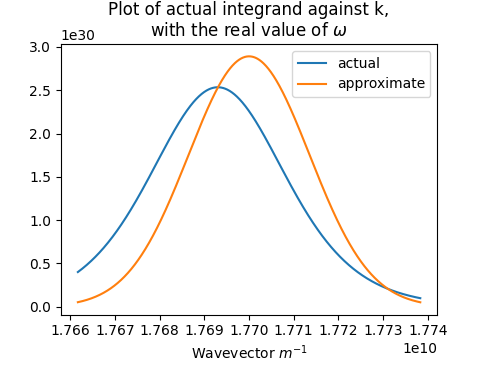
\includegraphics[width =0.9 \linewidth]{Figures/Redfield/real omega fermi k expansion.png}
        \caption{Approximation for Experimental \(\omega \)
        }\label{sub@fig:omega zero expansion}
    \end{subfigure}
    \hfill
    \begin{subfigure}{0.45\linewidth}
        \centering
        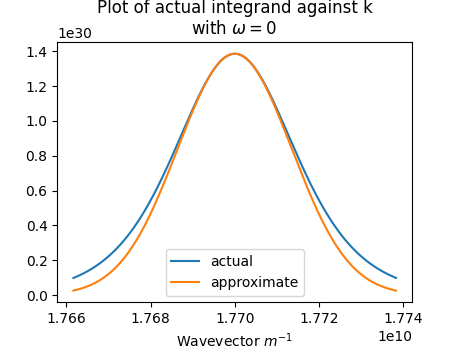
\includegraphics[width = 0.9\linewidth]{Figures/Redfield/zero omega fermi k expansion.png}
        \caption{Approximation for \(\omega = 0\)
        }\label{sub@fig:omega not zero expansion}
    \end{subfigure}
    \caption{
        Plot of the expansion of
        the integrand for \(\omega = 0\)
        (\cref{sub@fig:omega zero expansion})
        and the experimental \(\omega \)
        (\cref{sub@fig:omega not zero expansion}).
        Although the form of the
        integrand is shifted for the
        real value of \(\omega \)
        if we were to calculate
        the integrals we find
        they agree
        to within \(3\% \).
    }\label{fig:expansion about kf}
\end{figure}
the approximation
of the integral comes
to within \(3\% \)
of the true value.
If we apply this approximation
we find
\begin{equation}
    \Gamma_{i,j, k,l}(\omega_{k,l}) =\begin{aligned}[t]
        \sum_{s^1,s^3} \exp{(\frac{\beta \omega_{k,l}}{2})} \frac{m_e k_f^2 }{{(2\pi)}^4}
        V_{i,j} V_{k,l} \sqrt{\pi} \frac{2m_e}{\beta \hbar^2}
    \end{aligned}
\end{equation}
substituting in the expression
for \(V_{i,j}\)
we arrive at the final
expression for \(\Gamma \)
\begin{equation}
    \Gamma_{i,j, k,l}(\omega_{k,l})   =
    \exp{(\frac{\beta \omega_{k,l}}{2})}
    \mathcal{C}_{i,j} \mathcal{C}_{k,l}
    \sqrt{\pi} \frac{32 k_f^2 \epsilon_0^2 \hbar^3}{\beta e^4 {m_e}^2}
\end{equation}


\subsection{Two Sites}
Since the form of the rotating
wave approximation is a simple
rate equation, for a system
with one HCP and one FCC site
it is possible to solve it analytically
(\cref{app:combined tunnelling rates}).
From the expression above we find the
forward and backward tunnelling rate
\begin{align}
    \gamma_0 & = 2\Gamma_{1,0;0, 1}(\omega_{1,0})       \\
             & = A \exp{(\frac{\beta \omega_{0,1}}{2})}
    \mathcal{C}_{1,0} \mathcal{C}_{0,1}                 \\
    \gamma_1 & = 2\Gamma_{0,1;1, 0}(\omega_{0,1})       \\
             & = A \exp{(\frac{\beta \omega_{1,0}}{2})} \\
\end{align}
where
\(A =
\mathcal{C}_{1,0} \mathcal{C}_{0,1}
\sqrt{\pi}
\frac{64 k_f^2 \epsilon_0^2 \hbar^3}{\beta e^4 m_e^2}\).
This gives a combined rate of
\begin{equation}
    \gamma_0 + \gamma_1 = 2A\cosh{(\frac{\beta (E_1 - E_0)}{2})}
    \label{eqn:theoretical rate lindblad equation}
\end{equation}
for an energy difference of
\(3.04\pm0.16\times{}10^{-21} J\)
(\cref{eqn:hydrogen energy difference})
we find a tunnelling rate of
\(6.1\times{}10^{8}s^{-1}\),
corresponding to a
tunnelling time of
\(1.6\times{}10^{-9}s\) at
\(150K\).


\begin{figure}
    \centering
    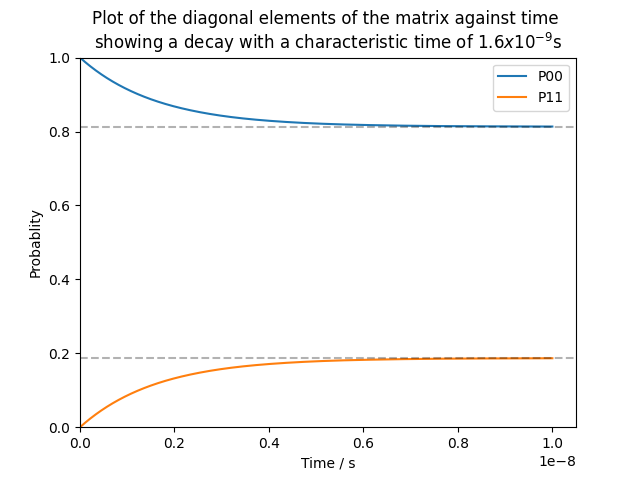
\includegraphics[width=.5\linewidth]{Figures/Redfield/Plot of lindblad solution.png}
    \caption{Plot of the Lindblad solution with a characteristic decay
    rate of \(6.1\times{}10^{8}s^{-1}\) at
    \(150K\).
    }\label{fig:two site lindblad soluton}
\end{figure}


\subsection{Multiple Sites}
In reality there
are 3 HCP sites neighbouring
each FCC Hydrogen, all of which
are connected to \(3\) HCP sites
(see \cref{sec:the model}).
The rate that the FCC
and HCP
occupation reaches the
boltzmann distribution
is therefore exactly \(3\)
times the single neighbour rate
(\cref{fig:multi site lindblad})
\begin{equation}
    R = 6A\cosh{(\frac{\beta (E_1 - E_0)}{2})}
\end{equation}
where \(R=1.8\times{}10^{9}s^{-1}\) at
\(150K\).
\begin{figure}[htbp]
    \centering
    \begin{subfigure}{0.45\linewidth}
        \centering
        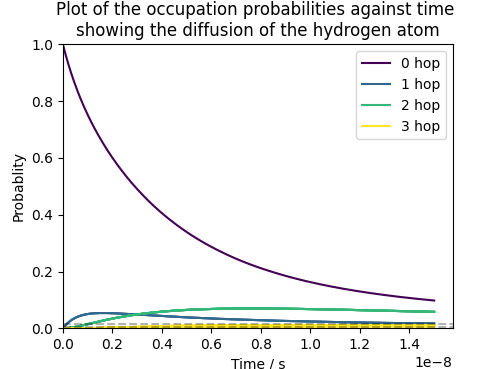
\includegraphics[width =0.9 \linewidth]{Figures/Redfield/Plot of lindblad solution many sites.png}
        \caption{Individual occupation probability
        }\label{sub@fig:multi site lindblad}
    \end{subfigure}
    \hfill
    \begin{subfigure}{0.45\linewidth}
        \centering
        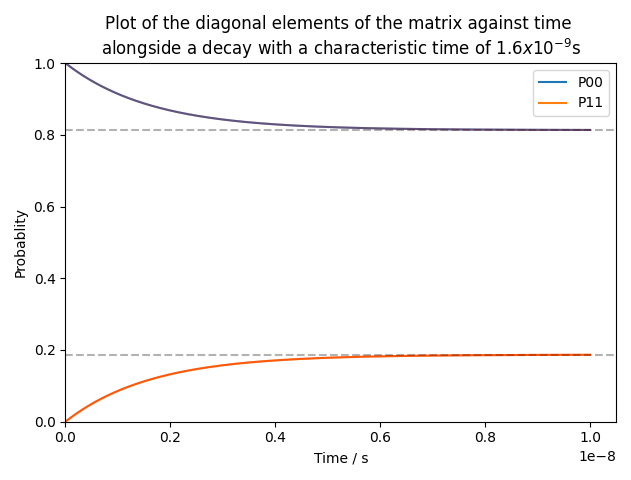
\includegraphics[width = 0.9\linewidth]{Figures/Redfield/Plot of redfield solution long time.png}
        \caption{Combined occupation probability
        }\label{sub@fig:multi site combined lindblad}
    \end{subfigure}
    \caption{Plot of the individual and combined
    occupation probabilities against time at
    \(150K\). The combined
    probability
    (\cref{sub@fig:multi site combined lindblad})
    follows exactly the same curve as in
    \cref{fig:two site lindblad soluton}
    with a rate of \(1.8\times{}10^{9}s^{-1}\).
    The plot of the individual occupation
    probabilities
    (\cref{sub@fig:multi site lindblad})
    shows that it takes
    a much longer time for the
    probability of occupation of the
    initial site to reach
    an equilibrium with the surroundings.}\label{fig:multi site lindblad}
\end{figure}
It is also possible to infer a
tunneling rate from the
individual probability
distribution
(\cref{sub@fig:multi site lindblad}),
where we take the tunneling
time as the time taken for the
distance from equilibrium
to fall by \(\exp{(-1)}\).
For the initial
FCC site we can
take this equilibrium
value to be zero,
or the boltzmann equilibrium.
We can also
use the time taken for the
neighbouring HCP sites to
reach their maximum occupation,
and half the time taken for the
neighbouring FCC to reach equilibrium.
The corresponding decay times are
given in \cref{tab:implied decay rates}.
\begin{table}[htbp]
    \begin{center}
        \begin{tabular}{ *{3}{c} }
            \toprule
            Measure                 & Decay Time \(s\)                   & Implied Decay Rate \(s^{-1}\) \\
            \midrule
            Initial FCC             & \(4.54\times{}10^{-9}\)            & \(2.2\times{}10^{8}\)         \\
            Initial FCC (Boltzmann) & \(3.99\times{}10^{-10}\)           & \(2.5\times{}10^{9}\)         \\
            Next HCP                & \(4.37\times{}10^{-10}\)           & \(2.3\times{}10^{9}\)         \\
            Next FCC                & \(4\times{}6.55 \times{}10^{-10}\) & \(1.5\times{}10^{9}\)         \\
            Combined Occupation     & \(5.56\times{}10^{-10}\)           & \(1.8\times{}10^{9}\)         \\
            RMS Distance            & \(5.09\times{}10^{-10}\)           & \(2.0 \times 10^{9}\)         \\
            \bottomrule
        \end{tabular}
    \end{center}
    \caption{Implied decay rates
        from the probability
        distribution and RMS distance
        analysis at
        \(150K\).
        Since the individual
        probabilities undergo an exponential
        decay we take the decay time as
        the time for the probability to fall
        by \(\exp{(-1)}\).
        The RMS decay time corresponds
        to the time for the RMS distance
        to equal \(0.5\).
        The implied decay time taken for
        the next FCC site is taken to
        be \(4\times \) the time to
        equilibrium, as the time
        taken grows as distance
        squared.
        Most measures
        of the decay rate take a similar
        amount of time, however the
        complete decay of the FCC
        occupation takes an order of
        magnitude longer.
    }\label{tab:implied decay rates}
\end{table}

\subsection{Distance Traveled}
We should also be able to
extract a tunneling time from
the root-mean squared (rms)
distance travelled by the
hydrogen. As the hydrogen
undergoes a random walk we should
expect the squared distance to
grow linearly with time.
\begin{figure}
    \centering
    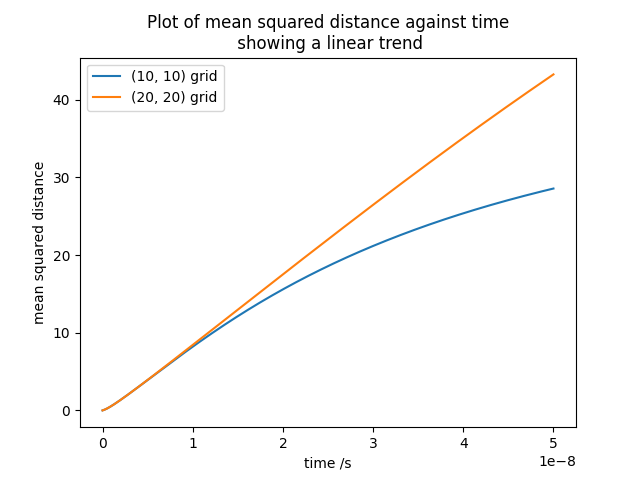
\includegraphics[width=0.5\linewidth]{Figures/Redfield/Plot of lindblad solution squared distance.png}
    \caption{Plot of the squared distance
    of the hydrogen atom against time
    showing a linear trend as expected
    for a random walk. The time taken
    for the rms distance to equal \(0.5\)
    is found to be
    \(5.09\times{}10^{-10}s\),
    which corresponds to an implied rate
    of \(2.0 \times 10^{9}s^{-1}\).
    }
\end{figure}
The tunneling time was
found to be \(5.25\times{}10^{-10}s\),
corresponding to the time taken
for the rms distance to
reach \(0.5\). This gives
an overall rate of
\(1.9 \times 10^{9}s^{-1}\).

\subsection{Comparison with Experiment}
Given these measures of the
tunneling time it is now possible to compare
these tunneling rates to experiment.
In \cref{fig:tunneling rate against temperature}
the theoretical rates
are plotted against temperature
alongside the rates extracted
from the Lindblad analysis.
\begin{figure}[htbp]
    \centering
    \begin{subfigure}{0.45\linewidth}
        \centering
        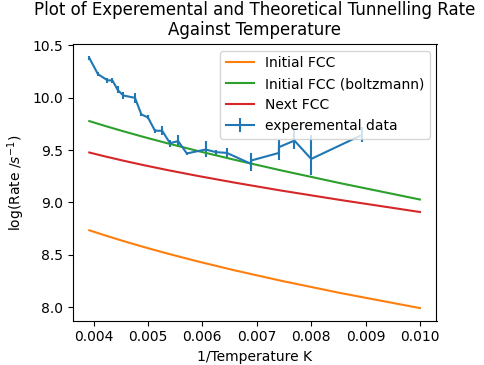
\includegraphics[width =0.9 \linewidth]{Figures/Redfield/Plot of redfield temperature dependance FCC points.png}
        \caption{FCC Tunneling Rates
        }\label{sub@fig:fcc tunneling rates temp dependence}
    \end{subfigure}
    \hfill
    \begin{subfigure}{0.45\linewidth}
        \centering
        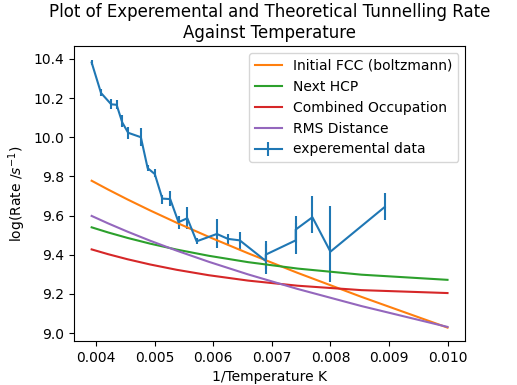
\includegraphics[width = 0.9\linewidth]{Figures/Redfield/Plot of redfield temperature dependance close points.png}
        \caption{Other Tunneling Rates
        }\label{sub@fig:other tunneling rates temp dependence}
    \end{subfigure}
    \caption{Plot of the tunneling
        rates against temperature, with comparison
        to the experimental data.
        The Initial FCC tunneling rate
        (\cref{sub@fig:fcc tunneling rates temp dependence})
        deviates significantly from the experimental
        measurements, however all other measures
        provide a close fit.
        The temperature dependance
        is significantly different
        depending on the
        property measured
        in the simulation
        (\cref{sub@fig:other tunneling rates temp dependence})
        although it is unclear
        which provides the
        closest fit to the data.
    }\label{fig:tunneling rate against temperature}
\end{figure}
Although the FCC tunneling
rates differ by an order of
magnitude the remaining
measurements of the rate
are similar to that measured
in experiment.
TODO-Temp dependance discussion
